\chapter{Пересчет динамических приоритетов}
В ОС семейства Windows и Unix/Linux только приоритеты пользовательских процессов могут динамически пересчитываться.

\section{Пересчет динамических приоритетов в ОС семейства Windows}
В ОС семейства Windows при создании процесса ему назначается базовый приоритет; относительно него потоку назначается относительный приоритет.

Планирование осуществляется на основании приоритетов потоков, готовых к выполнению. Планировщик вытесняет поток с более низким приоритетом, когда поток с более высоким приоритетом становится готовым к выполнению. По истечении кванта времени текущего потока ресурс передается первому потоку (с наибольшим приоритетом) в очереди готовых на выполнение.

Диспетчер настройки баланса выполняет сканирование очереди готовых потоков раз в секунду. Если обнаружены потоки, которые ожидают выполнение более четырех секунд, то диспетчер повышает их приоритет до пятнадцати. Как только квант процессорного времени истекает, приоритет потока снижается до базового. Если поток не был завершен за этот квант или был вытеснен потоком с более высоким приоритетом, то выполняется снижение приоритета и поток возвращается в очередь готовых потоков. Для минимизации расхода процессорного времени диспетчер настройки баланса сканирует лишь шестнадцать готовых потоков. Кроме того он повышает приоритет не более чем у десяти потоков за один проход. Если обнаружено десять потоков, приоритет которых необходимо повысить, то сканирование прекращается. При следующем проходе оно возобновляется с того места, где было прервано в прошлый раз. Наличие десяти потоков, приоритет которых следует повысить, говорит о необычайной загруженности системы.

В операционных системах семейства Windows используется 32 уровня приоритета, от 0 до 31, как показано на рисунке \ref{png:priority}:

\begin{figure}[H]
	\centering
	{
		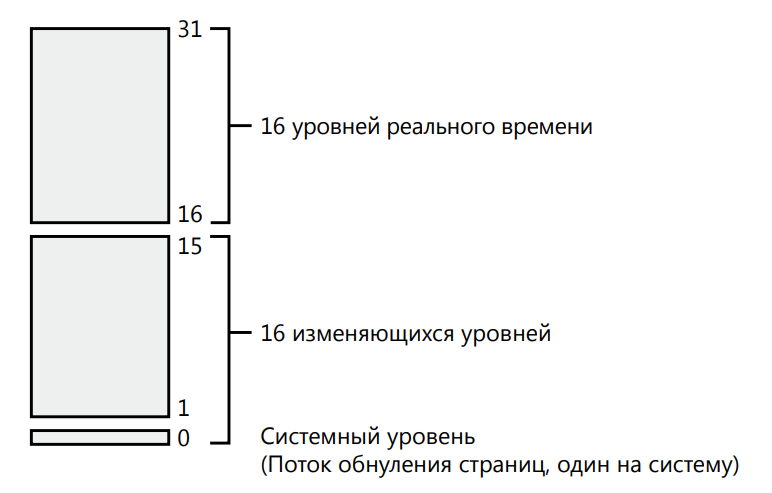
\includegraphics[scale=0.9]{../../../../../../../msys64/home/Лев/bmstu_sem_5_os/lab_01/part_2/report/images/priority}
		\caption{Уровни приоритета потоков.}
		\label{png:priority}
	}
\end{figure}

Уровни приоритета потоков назначаются Windows API и ядром операционной системы. Сначала Windows API систематизирует процессы по классу приоритета, который присваивается им при их создании:
\begin{itemize}
	\item реального времени (real-time) - 4;
	\item высокий (high) - 3;
	\item выше обычного (above normal) - 7;
	\item обычный (normal) - 2; 
	\item ниже обычного (below normal) - 5;
	\item простой (idle) - 1.
\end{itemize}
 
Затем назначается относительный приоритет потоков в рамках процессов:
\begin{itemize}
	\item критичный по времени (real-time) - 15;
	\item наивысший (high) - 2;
	\item выше обычного (above normal) - 1;
	\item обычный (normal) - 0; 
	\item ниже обычного (below normal) - -1;
	\item низший (lowest) - -2;
	\item простой (idle) - -15.
\end{itemize}

Исходный базовый приоритет потока наследуется от базового приоритета процесса. Процесс по умолчанию наследует свой базовый приоритет у того процесса, который его создал. 

Соответствие между приоритетами Windows API и ядра системы приведено на рисунке \ref{png:table_priority_windows}:
\begin{figure}[H]
	\centering
	{
		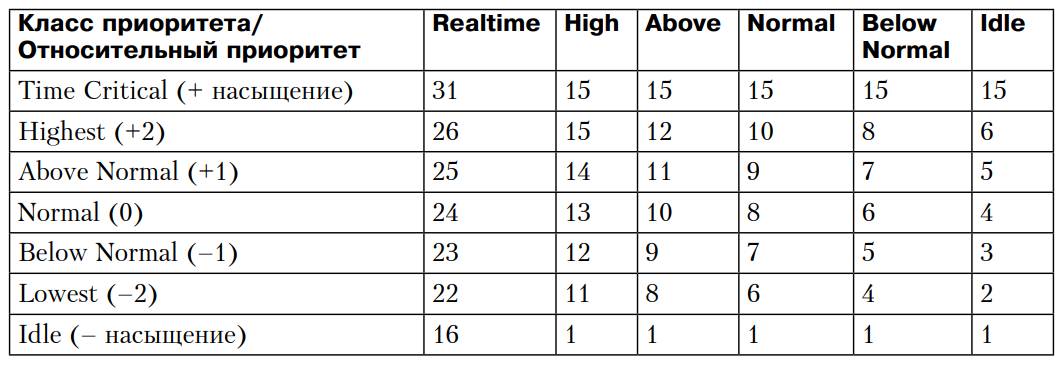
\includegraphics[scale=0.7]{../../../../../../../msys64/home/Лев/bmstu_sem_5_os/lab_01/part_2/report/images/table_priority_windows}
		\caption{Уровни приоритета потоков.}
		\label{png:table_priority_windows}
	}
\end{figure} 

Текущий приоритет потока в динамическом диапазоне (от 1 до 15) может быть повышен планировщиком вследствие следующих причин:
\begin{itemize}
	\item вследствие события планировщика или диспетчера;
	\item повышение приоритета владельца блокировки; 
	\item после завершения ввода/вывода (см. таблицу \ref{tab:io});
	\item вследствие ввода из пользовательского интерфейса;
	\item длительного ожидания ресурса исполняющей системы;
	\item вследствие ожидания объекта ядра;
	\item в случае, когда готовый к выполнению поток не был запущен в течение длительного времени;
	\item проигрывание мультимедиа службой планировщика MMCSS.	 
\end{itemize} 

Текущий приоритет потока в динамическом диапазоне может быть понижен до базового путем вычитания всех повышений.

\begin{table}[ht!]
	\captionsetup{singlelinecheck = false, justification=raggedright}
	\caption{Рекомендуемые значения повышения приоритета.}
	\begin{center}
		\begin{tabular}{|p{100mm}|l|}
			\hline
			\textbf{Устройство} & \textbf{Приращение} \\
			\hline
			Диск, CD-ROM, параллельный порт, видео & 1 \\
			\hline
			Сеть, почтовый ящик, именованный канал, последовательный порт & 2 \\
			\hline
			Клавиатура, мышь & 6 \\
			\hline
			Звуковая плата & 8 \\
			\hline
		\end{tabular}
	\end{center}
	\label{tab:io}
\end{table}

\subsection{MMCSS}
Мультимедийные потоки должны выполняться с минимальными задержками. Повышение приоритета проигрывания обычно выполняется службой пользовательского режима - служба планировщика класса мультимедиа (Multimedia Class Scheduler Service). MMCSS работает со следующими задачами:
\begin{itemize}
	\item аудио;
	\item захват;
	\item распределение;
	\item игры;
	\item проигрывание;
	\item аудио профессионального качества;
	\item задачи администратора многооконного режима.	
\end{itemize}

Каждая из этих задач включает информацию о свойствах, которые отличаются друг от друга. Одним из наиболее важным свойством для планирования потоков является категория планирования (scheduling category). Она является первичным фактором, который определяет приоритет потоков, зарегистрированных с MMCSS. На рисунке \ref{png:category_plans} показаны различные категории планирования:
\begin{figure}[H]
	\centering
	{
		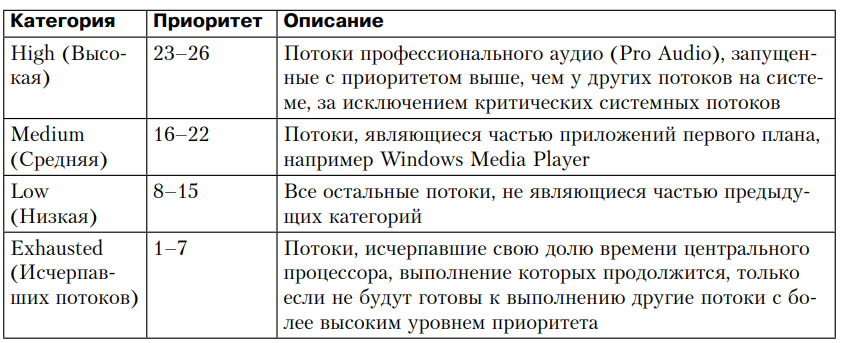
\includegraphics[scale=0.9]{../../../../../../../msys64/home/Лев/bmstu_sem_5_os/lab_01/part_2/report/images/plan_categories}
		\caption{Категории планирования.}
		\label{png:category_plans}
	}
\end{figure}

Механизм, положенный в основу MMCSS, повышает приоритет потоков внутри зарегистрированного процесса до уровня, соответствующего их категории планирования. Затем он снижает категорию этих потоков до exhausted, чтобы другие, которые не относятся к мультимедийным приложениям, могли получить ресурс.

\section{Пересчет динамических приоритетов в ОС семейства Unix/Linux}
В современных системах Unix/Linux в режиме ядра процесс может быть вытеснен более приоритетным процессом. Ядро было сделано вытесняющим для того, чтобы система могла обслуживать процессы реального времени, такие как аудио, видео.

Очередь готовых к выполнению процессов формируется согласно приоритетам процессов и принципу вытесняющего циклического планирования: в первую очередь выполняются процессы с большим приоритетом. Если процессы имеют одинаковый приоритет, то они выполняются в течение кванта времени циклически друг за другом. Если в очередь готовых к выполнению поступает процесс, который имеет более высокий приоритет, то планировщик вытесняет текущий процесс и предоставляет ресурс более приоритетному.

Приоритет представляет собой целое число из диапазона от 0 до 127 (чем меньше число, тем выше приоритет):
\begin{itemize}
	\item в диапазоне от 0 до 49 находятся приоритеты ядра;
	\item в диапазоне от 50 до 127 - приоритеты прикладных задач.
\end{itemize}

Приоритеты прикладных задач могут изменяться во времени в зависимости от следующих двух факторов:
\begin{itemize}
	\item фактор любезности;
	\item последней измеренной величиной использования процесса.
\end{itemize}

Фактор любезности - целое число в диапазоне от 0 до 39 со значением 20 по умолчанию. С увеличением фактора любезности происходит уменьшение приоритета процесса. Фоновым процессам автоматически задаются более высокие значения этого фактора. Фактор любезности может быть изменен суперпользователем при помощи системного вызова nice().

На рисунке \ref{png:priority_unix} приведены поля структуры proc, относящиеся к приоритетам:
\begin{figure}[H]
	\centering
	{
		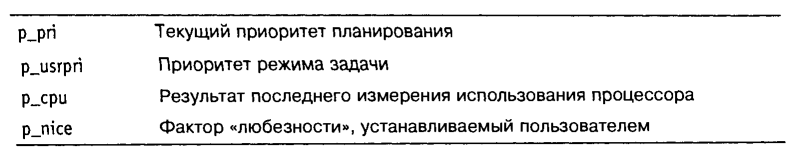
\includegraphics[scale=0.9]{../../../../../../../msys64/home/Лев/bmstu_sem_5_os/lab_01/part_2/report/images/priority_unix}
		\caption{Поля структуры proc, относящиеся к приоритетам.}
		\label{png:priority_unix}
	}
\end{figure}

Планировщик использует p\_pri для принятия решения о том, какой процесс направить на выполнение. У процесса, находящего в режиме задачи, значения p\_pri и p\_usrpri идентичны. Значение текущего приоритета p\_pri может быть повышено планировщиком для выполнения процесса в режиме ядра. В таком случае p\_usrpri будет использоваться для хранения приоритета, который будет назначен процессу при возврате в режим задачи. 

Ядро системы связывает приоритет сна с событием или ожидаемым ресурсом, из-за которого процесс может блокироваться. Когда процесс просыпается после блокирования в системном вызове, ядро устанавливает в поле p\_pri приоритет сна - значение приоритета из диапазона от 0 до 49, зависящее от события или ресурса, по которому произошла блокировка.

При создании процесса поле p\_cpu инициализируется нулем. НА каждом тике обработчик таймера увеличивает поле p\_cpu текущего процесса на единицу до максимального значения, равного 127. Каждую секунду обработчик прерывания инициализирует отложенный вызов процедуры schedcpy(), которая уменьшает значение p\_cpu каждого процесса исходя из фактора \grqqполураспада\grqq. В системе 4.3BSD для расчета фактора полураспада используется формула (\ref{for:bsd}):
\begin{equation}
	\label{for:bsd}
	decay = \frac{2 \cdot load\_average}{2 \cdot load\_average + 1}
\end{equation}
где load\_average - среднее количество процессов, которые находятся в состоянии готовности к выполнению, за последнюю секунду.

Процедура schedcpy() пересчитывает приоритеты для режима задачи всех процессов по формуле (\ref{for:sc}):
\begin{equation}
	\label{for:sc}
	p\_usrpri = PUSER + \frac{p\_cpu}{2} + 2 \cdot p\_nice
\end{equation}
где PUSER - базовый приоритет в режиме задачи, равный 50. 

В результате, если процесс в последний раз процесс использовал большое количество процессорного времени, то его p\_cpu будет увеличен. Это приведет к росту значения поля p\_usrpri и, следовательно, к понижению приоритета. Чем дольше процесс простаивает в очереди на исполнение, тем больше фактор полураспада уменьшает его p\_cpu; это приводит к повышению его приоритета. Такая схема предотвращает зависание низкоприоритетных процессов по вине операционной системы. Её применение предпочтительнее процессам, которые осуществляют множество операций ввода-вывода, в противоположность тем, которые производят много вычислений.